\documentclass[12pt, a4paper]{article}
\usepackage{enumitem}
\usepackage{float}
\usepackage[left=2cm, right=2cm, top=2cm, bottom=2cm]{geometry}
\usepackage{graphicx}
\usepackage[colorlinks, urlcolor=blue]{hyperref}
\usepackage{minted}
\usepackage{xeCJK}

\renewcommand\arraystretch{1.1}
\setCJKmainfont[AutoFakeBold=1.5]{新細明體}

\setminted{
  frame=single,
}

\title{
  \vspace{-1cm}
  Network Administration/System Administration\\
  (NTU CSIE, Spring 2024)\\
  Homework \#7
}
\author{\Large B12902110 呂承諺}

\begin{document}
  \maketitle

  \section{Do you know what is DNS?}
  \begin{enumerate}
    \item DNS stands for Domain Name System. It is a naming system for
    hosts and services in the Internet. It manages various information
    associated with a domain name, such as its IP address, aliases, name servers, etc.

    \textbf{References}
    \begin{itemize}
      \item \href{https://en.wikipedia.org/wiki/Domain_Name_System}{Domain Name System - Wikipedia}
      \item \href{https://www.cloudflare.com/learning/dns/what-is-dns/}{Dynamic DNS | Cloudflare}
    \end{itemize}

    \item DDNS stands for Dyanmic DNS. It is a service that that automatically
    updates DNS records when an IP address of the service or resource changes.

    \textbf{References}
    \begin{itemize}
      \item \href{https://www.cloudflare.com/learning/dns/glossary/dynamic-dns/}{Dynamic DNS | Cloudflare}
    \end{itemize}

    \item There are 13 root name servers.

    \textbf{References}
    \begin{itemize}
      \item \href{https://en.wikipedia.org/wiki/Root_name_server}{Root name server - Wikipedia}
    \end{itemize}

    \item An example is the Sender Policy Framework (SPF). It list all the servers
    that are authorized to send email messages from a domain. Email receivers can then
    compare the SPF information with the email's header to confirm the email is sent
    from a reliable source. This is needed because SMTP allows any computer to send
    email claiming to be any source address, which could lead to spamming or phishing.

    \textbf{References}
    \begin{itemize}
      \item \href{https://en.wikipedia.org/wiki/Sender_Policy_Framework}{Sender Policy Framework - Wikipedia}
      \item \href{https://www.cloudflare.com/learning/dns/dns-records/dns-txt-record/}{What is a DNS TXT record? | Cloudflare}
    \end{itemize}
  \end{enumerate}

  \pagebreak
  \section{Do you know how to reach CSIE DNS?}
  \begin{minted}{shell}
$ dig +trace -4 www.csie.ntu.edu.tw
  \end{minted}

  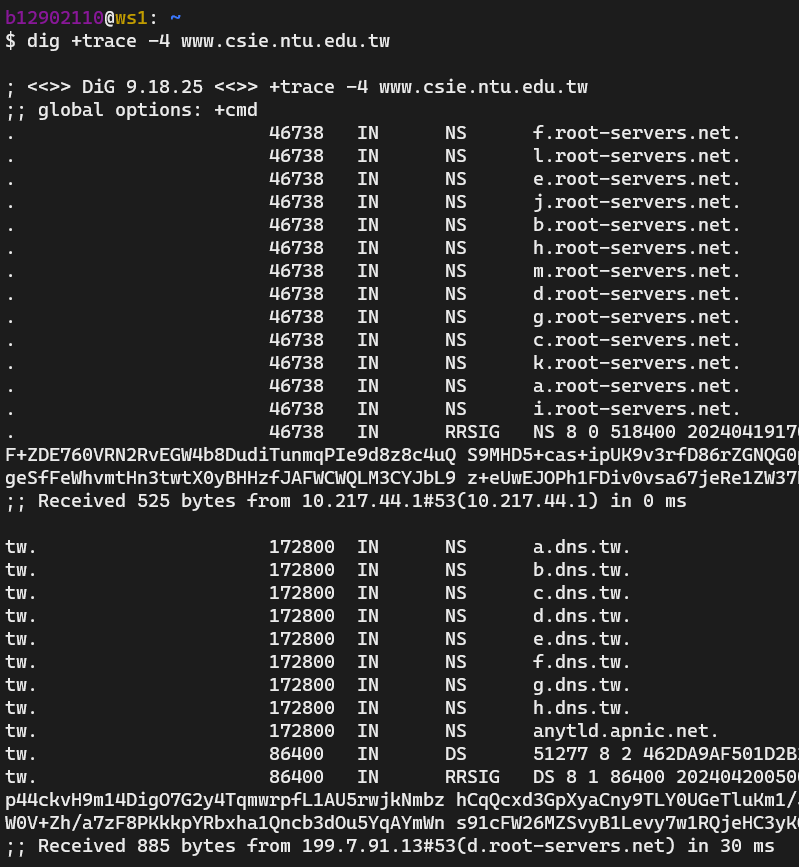
\includegraphics[width=0.9\textwidth]{2_dig_trace_1.png}

  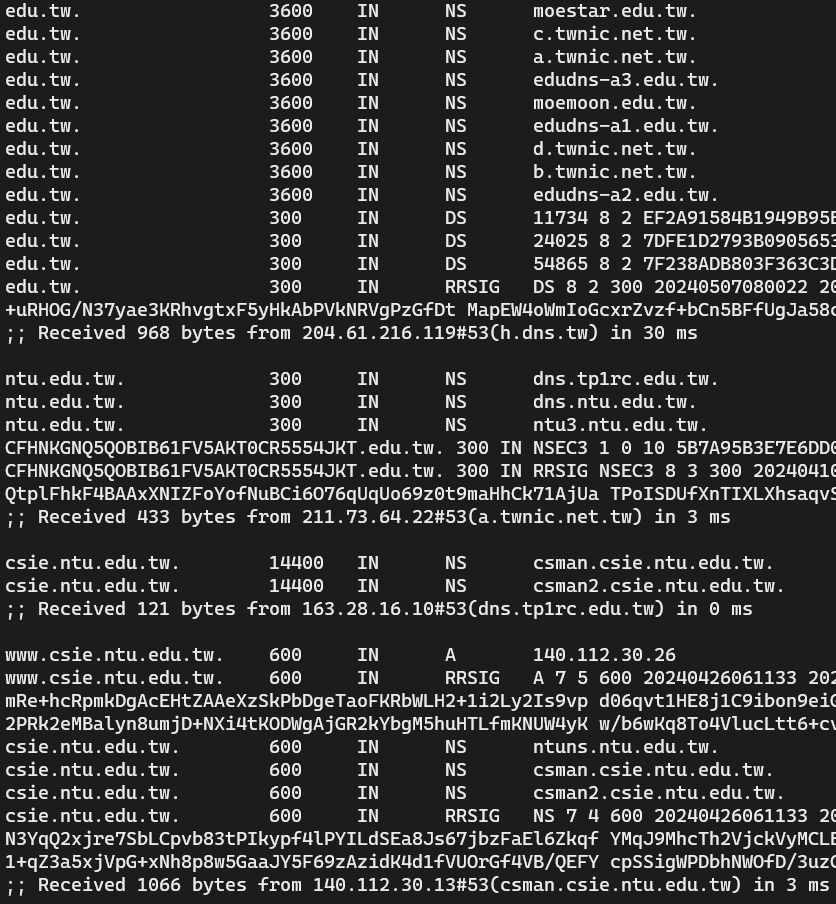
\includegraphics[width=0.9\textwidth]{2_dig_trace_2.png}

  \begin{table}[H]
    \centering
    \begin{tabular}{|c|c|c|}
      \hline
      \textbf{Domain Name} & \textbf{IP address} & \textbf{Zone} \\\hline
      d.root-servers.net & 199.7.91.13 & Root \\
      h.dns.tw & 204.61.216.119 & tw \\
      a.twnic.net.tw & 211.73.64.22 & edu.tw \\
      dns.tp1rc.edu.tw & 163.28.16.10 & ntu.edu.tw \\
      csman.csie.ntu.edu.tw & 140.112.30.13 & csie.ntu.edu.tw \\
      www.csie.ntu.edu.tw & 140.112.30.26 & N/A \\\hline
    \end{tabular}
  \end{table}

  \textbf{References}
  \begin{itemize}
    \item \href{https://superuser.com/questions/715632/how-does-dig-trace-actually-work}{dns - How does dig +trace actually work? - Super User}
  \end{itemize}

  \pagebreak
  \section{Do you know how to design a DNS architecture?}

  \begin{itemize}
    \item Basic DNS server setup:
    \begin{itemize}
      \item Setup a DNS server, perferably with a static IP address \verb|xxx.xxx.xxx.xxx|.
      \item Register the following records to the authoritative servers of zone \verb|ntu.edu.tw|.

      (Zone: \verb|ntu.edu.tw|)

      \begin{tabular}{|c|c|c|}
        \hline
        \textbf{Name} & \textbf{Type} & \textbf{Data} \\\hline
        \verb|csie| & NS & \verb|ns.csie.ntu.edu.tw.| \\
        \verb|ns.csie| & A & \verb|xxx.xxx.xxx.xxx| \\\hline
      \end{tabular}
    \end{itemize}
    \item
    Q:如果今天其中一台伺服器壞掉了怎麼辦?

    A:
    Maintain multiple mirror servers, and register multiple NS and A records
    to the authoritative servers of zone \verb|ntu.edu.tw|.

    (Zone: \verb|ntu.edu.tw|)

    \begin{tabular}{|c|c|c|}
      \hline
      \textbf{Name} & \textbf{Type} & \textbf{Data} \\\hline
      \verb|csie| & NS & \verb|ns1.csie.ntu.edu.tw.| \\
      \verb|csie| & NS & \verb|ns2.csie.ntu.edu.tw.| \\
      \verb|csie| & NS & \verb|ns3.csie.ntu.edu.tw.| \\
      \verb|ns1.csie| & A & \verb|xxx.xxx.xxx.xxx| \\
      \verb|ns2.csie| & A & \verb|yyy.yyy.yyy.yyy| \\
      \verb|ns3.csie| & A & \verb|zzz.zzz.zzz.zzz| \\\hline
    \end{tabular}

    \item Q:如果今天系館停電導致所有機房下線怎麼辦?

    A:Place at least one of the CSIE DNS servers elsewhere, such as in 計中
    or outside of NTU.

    \item Q:如果因為某些原因導致伺服器上的DNS records不見了怎麼辦?

    A:
    \begin{itemize}
      \item Regularly backup all configurations, including DNS records.
      \item Keep a log of all configuration changes.
    \end{itemize}

    \item Q:有些實驗室想要擁有自己的subdomain,該如何實現?

    A:Register NS and A records of the lab's DNS server to our DNS server.

    (Zone: \verb|csie.ntu.edu.tw|)

    \begin{tabular}{|c|c|c|}
      \hline
      \textbf{Name} & \textbf{Type} & \textbf{Data} \\\hline
      \verb|lab1| & NS & \verb|ns.lab1.csie.ntu.edu.tw.| \\
      \verb|ns.lab1| & A & \verb|xxx.xxx.xxx.xxx| \\
      \verb|lab2| & NS & \verb|ns.lab2.csie.ntu.edu.tw.| \\
      \verb|ns.lab2| & A & \verb|yyy.yyy.yyy.yyy| \\\hline
    \end{tabular}

    \pagebreak
    \item Q:如何應對DNS flooding attack?

    A:
    \begin{itemize}
      \item Limit the rate of queries from a single source.
      \item Limit repeated queries for nonexistent domains.
      \item Distribute DNS service across multiple servers.
    \end{itemize}

    \item Q:如何應對DNS amplification attack?

    A:
    \begin{itemize}
      \item Limit the rate of queries from a single source.
      \item Only provide service to the necessary networks.
      \item Reject traffic sent with the spoofed IP addresses.
    \end{itemize}

    \item Q:如何確保對*.csie.ntu.edu.tw 的query response 不會被攻擊者竄改成malicious ip 呢?

    A:Use DNSSEC or DNS over TLS.
  \end{itemize}

  \textbf{References}
  \begin{itemize}
    \item \href{https://serverfault.com/questions/764937/why-dont-ns-records-contain-ip-addresses}{domain name system - Why don't NS records contain IP addresses? - Server Fault}
    \item \href{https://www.cloudflare.com/learning/ddos/dns-flood-ddos-attack/}{What is a DNS flood? | DNS flood DDoS attack | Cloudflare}
    \item \href{https://www.catchpoint.com/dns-monitoring/dns-flood}{Understanding and Preventing DNS Flood Attacks}
    \item \href{https://www.cloudflare.com/learning/ddos/dns-amplification-ddos-attack/}{DNS amplification DDoS attack | Cloudflare}
  \end{itemize}

  \pagebreak
  \section{The Power of DNS}
  The operating system is Ubuntu 22.04.4 LTS. Assume that Docker is already
  installed and configured.

  \begin{enumerate}
    \item
    \textbf{Steps}
    \begin{enumerate}
      \item Install the required packages.
      \begin{minted}{shell}
$ sudo apt-get install -y \
    mysql-server pdns-server pdns-backend-mysql
      \end{minted}
      \item Run the following SQL commands:
      \begin{Verbatim}[frame=single]
$ sudo mysql
mysql> CREATE USER 'powerdns'@'localhost'
    -> IDENTIFIED BY 'powerdns-mysql-password';
Query OK, 0 rows affected (0.02 sec)
mysql> CREATE DATABASE powerdns;
Query OK, 1 row affected (0.20 sec)
mysql> GRANT ALL ON powerdns.* TO 'powerdns'@'localhost';
Query OK, 0 rows affected (0.16 sec)
mysql> exit
$ sudo mysql -u powerdns -p powerdns \
  < /usr/share/pdns-backend-mysql/schema/schema.mysql.sql
      \end{Verbatim}
      \item Change the following setting in \verb|/etc/powerdns/pdns.conf|:
      \begin{Verbatim}[frame=single]
launch=gmysql
gmysql-password=powerdns-mysql-password
      \end{Verbatim}
      \item Free up 53 port for the PowerDNS server.
      \begin{minted}{shell}
$ sudo systemctl stop systemd-resolved
      \end{minted}
      \item (Re)start the PowerDNS server.
      \begin{minted}{shell}
$ sudo systemctl restart pdns.service
      \end{minted}
    \end{enumerate}

    \pagebreak
    \textbf{Result}

    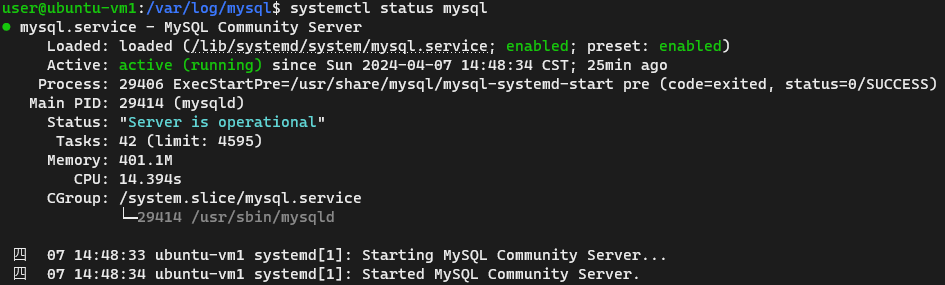
\includegraphics[width=0.93\textwidth]{4-1_status_mysql.png}

    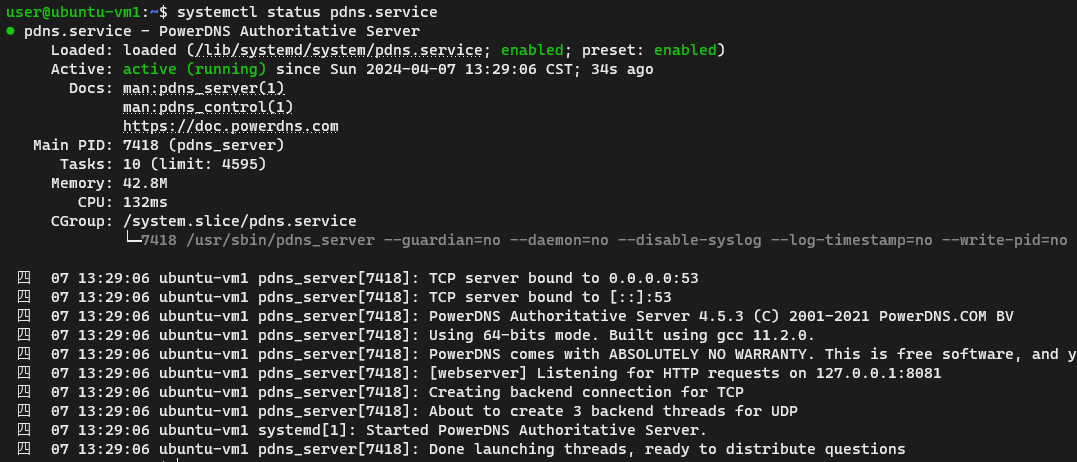
\includegraphics[width=0.93\textwidth]{4-1_status_pdns.png}

    \textbf{References}
    \begin{itemize}
      \item \href{https://doc.powerdns.com/authoritative/installation.html}{Installing PowerDNS — PowerDNS Authoritative Server  documentation}
      \item \href{https://packages.debian.org/search?keywords=pdns-backend}{Debian -- Package Search Results -- pdns-backend}
      \item \href{https://blog.steveyi.net/posts/ubuntu-53-port-already-in-use/}{解決 Ubuntu 上 53 Port 占用問題 | 小易的部落格}
      \item \href{https://doc.powerdns.com/authoritative/backends/index.html}{Backends — PowerDNS Authoritative Server  documentation}
      \item \href{https://doc.powerdns.com/authoritative/backends/generic-mysql.html}{Generic MySQL backend — PowerDNS Authoritative Server  documentation}
      \item \href{https://ubuntu.com/server/docs/databases-mysql}{Install and configure a MySQL server | Ubuntu}
      \item \href{https://stackoverflow.com/questions/41645309/mysql-error-access-denied-for-user-rootlocalhost}{sql - MySQL Error: : 'Access denied for user 'root'@'localhost' - Stack Overflow}
      \item \href{https://blog.hoyo.idv.tw/?p=10585}{PowerDNS - hoyo 學習紀錄}
    \end{itemize}

    \pagebreak
    \item
    \textbf{Steps}
    \begin{enumerate}
      \item Change the following settings in \verb|/etc/powerdns/pdns.conf|:
      \begin{Verbatim}[frame=single]
api=yes
api-key=b12902110-pdns-key
      \end{Verbatim}
      \item (Re)start the PowerDNS server.
      \begin{minted}{shell}
$ sudo systemctl restart pdns.service
      \end{minted}
      \item Verfiy that the PowerDNS API is configured properly:
      \begin{minted}{shell}
$ curl -H 'X-API-Key: b12902110-pdns-key' \
    http://127.0.0.1:8081/api/v1/servers/localhost/zones
      \end{minted}
      The output should be an empty array for now:
      \begin{Verbatim}[frame=single]
[]
      \end{Verbatim}
      \item Start the PowerDNS-Admin Docker container. Make sure to use host type network.
      \begin{minted}{shell}
$ sudo docker run -d \
    -e SECRET_KEY='b12902110-flask-key' \
    -e BIND_ADDRESS=0.0.0.0:9191 \
    -v pda-data:/data \
    --network=host \
    powerdnsadmin/pda-legacy:latest
      \end{minted}
      \item Go to the web interface of PowerDNS-Admin (\verb|http://localhost:9191/|) and create an account.

      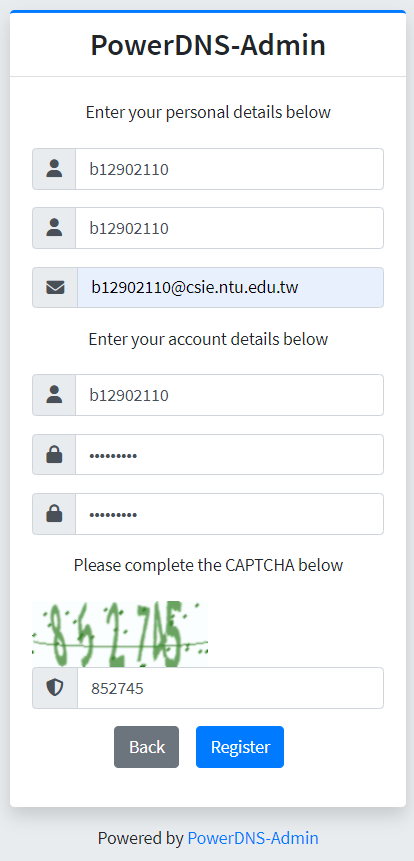
\includegraphics[width=0.3\textwidth]{4-2_create_account.png}

      \pagebreak
      \item Login and go to \textbf{Settings > Server}. Enter the following setting values:
      \begin{itemize}
        \item \textbf{PowerDNS API URL}: \verb|http://127.0.0.1:8081/|
        \item \textbf{PowerDNS API Key}: \verb|b12902110-pdns-key|
        \item \textbf{PowerDNS Version}: 4.5.3
      \end{itemize}

      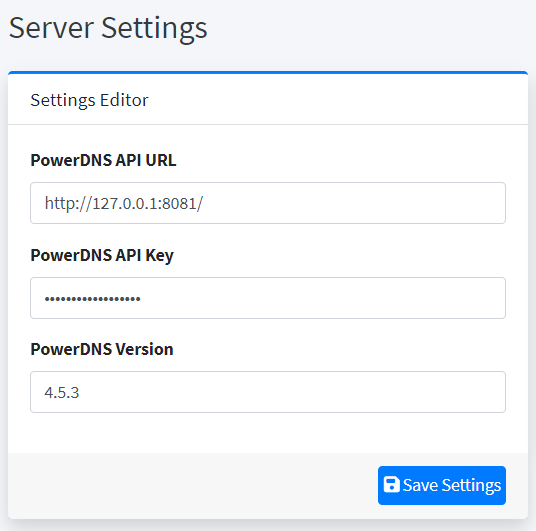
\includegraphics[width=0.45\textwidth]{4-1_server_settings.png}
    \end{enumerate}

    \textbf{Result} Go to \textbf{Server Configuration}. If the configurations show up,
    that means the API is configured successfully.

    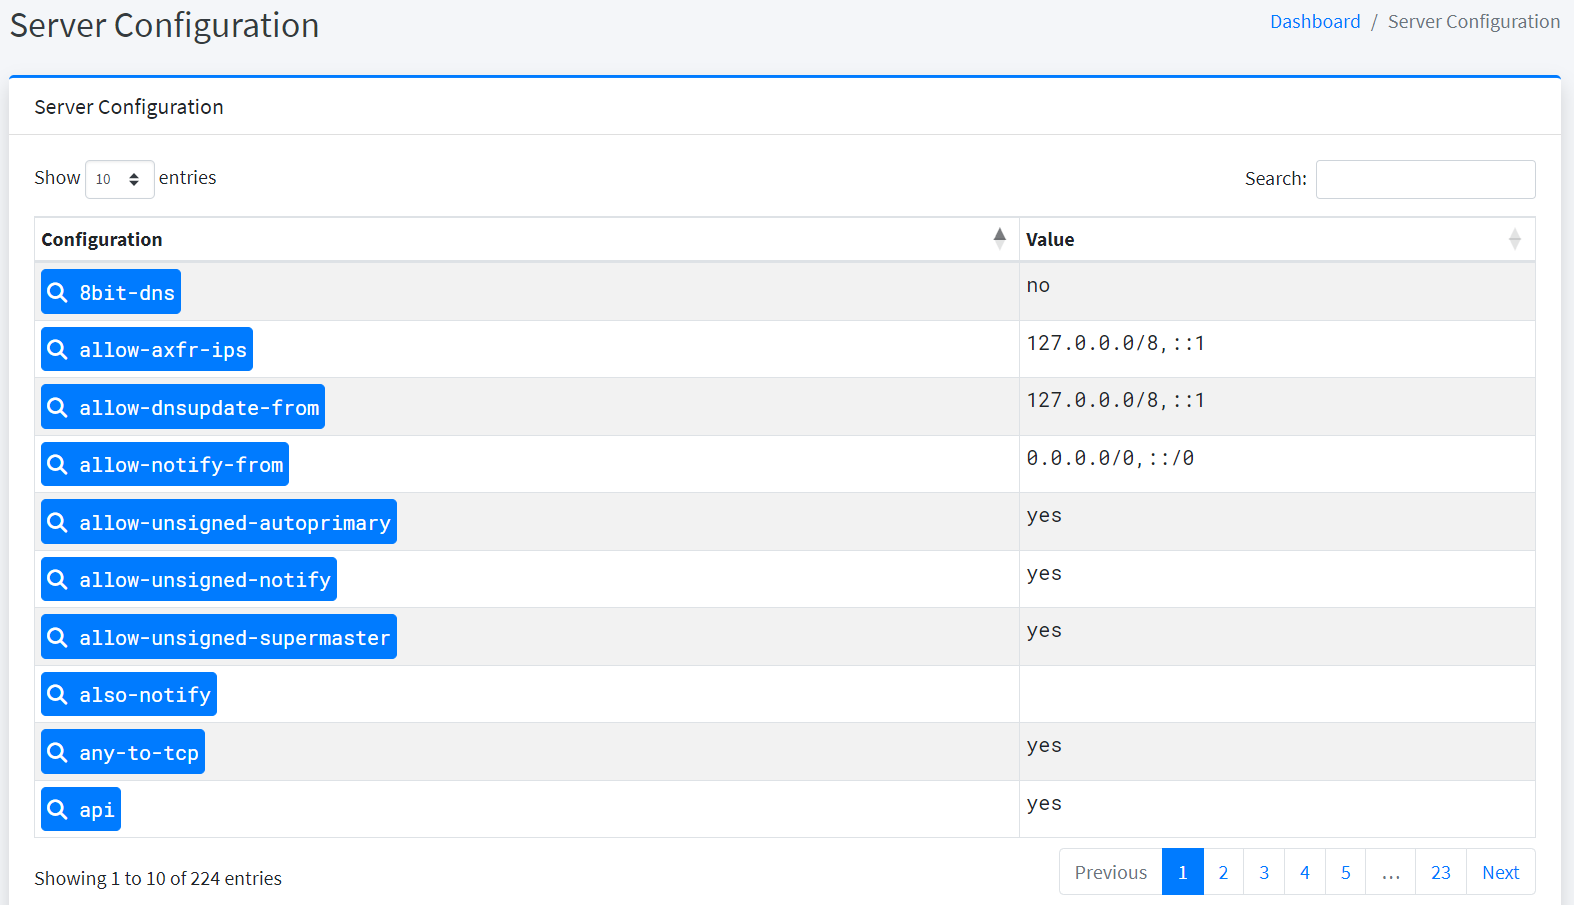
\includegraphics[width=0.8\textwidth]{4-2_server_configuration.png}

    \textbf{References}

    \begin{itemize}
      \item \href{https://github.com/PowerDNS-Admin/PowerDNS-Admin}{GitHub - PowerDNS-Admin/PowerDNS-Admin: A PowerDNS web interface with advanced features}
      \item \href{https://doc.powerdns.com/md/httpapi/README/}{HTTP API - Introduction}
      \item \href{https://doc.powerdns.com/authoritative/http-api/index.html}{Built-in Webserver and HTTP API — PowerDNS Authoritative Server  documentation}
      \item \href{https://github.com/PowerDNS-Admin/PowerDNS-Admin/blob/master/docs/wiki/configuration/Environment-variables.md}{PowerDNS-Admin/docs/wiki/configuration/Environment-variables.md at master · PowerDNS-Admin/PowerDNS-Admin · GitHub}
    \end{itemize}

    \pagebreak
    \item
    \textbf{Steps}
    \begin{enumerate}
      \item Go to \textbf{Create Zone} and create zone \verb|nasa.csie.tw|.

      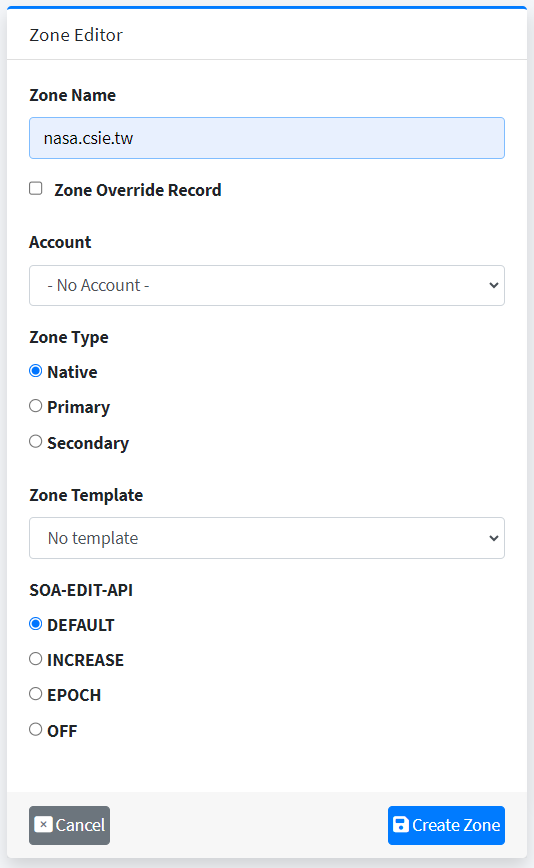
\includegraphics[width=0.45\textwidth]{4-3_create_zone.png}

      \item Go to \textbf{Zone Records - nasa.csie.tw} and create the following records.

      \begin{tabular}{|c|c|c|}
        \hline
        \textbf{Name} & \textbf{Type} & \textbf{Data}\\\hline
        \verb|*.sub| & NS & \verb|subns.nasa.csie.tw.| \\
        \verb|subns| & A & \verb|10.1.6.88| \\
        \verb|verification| & TXT & \verb|"I LOVE NASA"| \\\hline
      \end{tabular}

      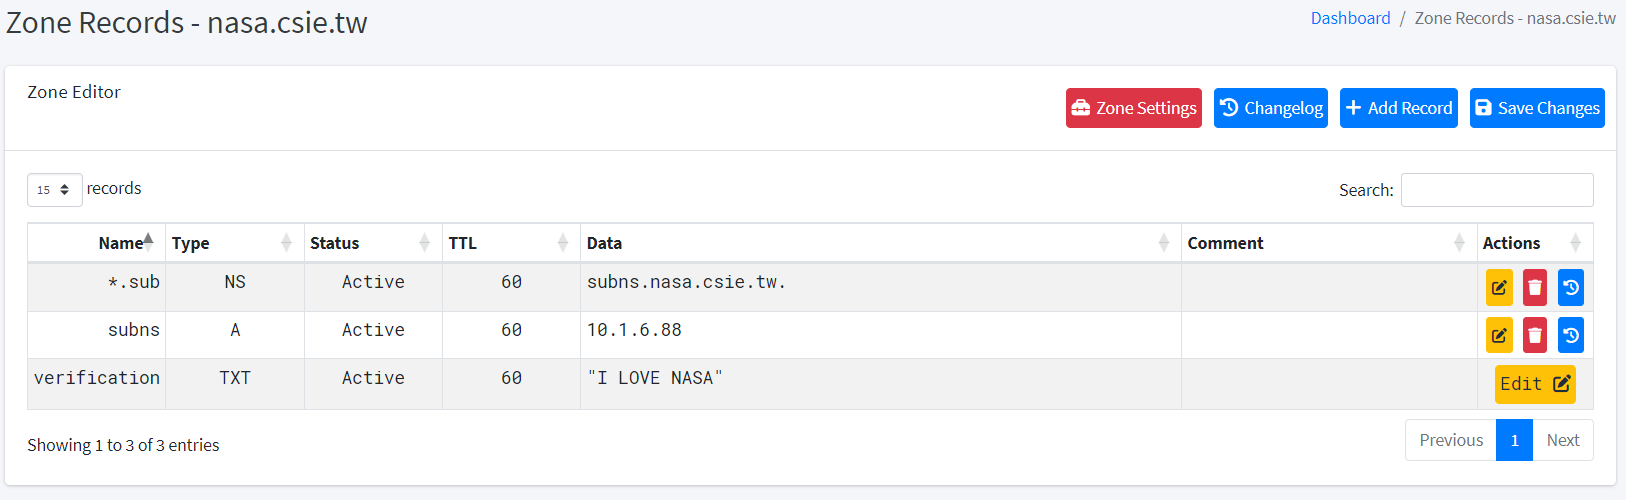
\includegraphics[width=0.9\textwidth]{4-3_zone_records.png}
    \end{enumerate}

    \pagebreak
    \textbf{Result}

    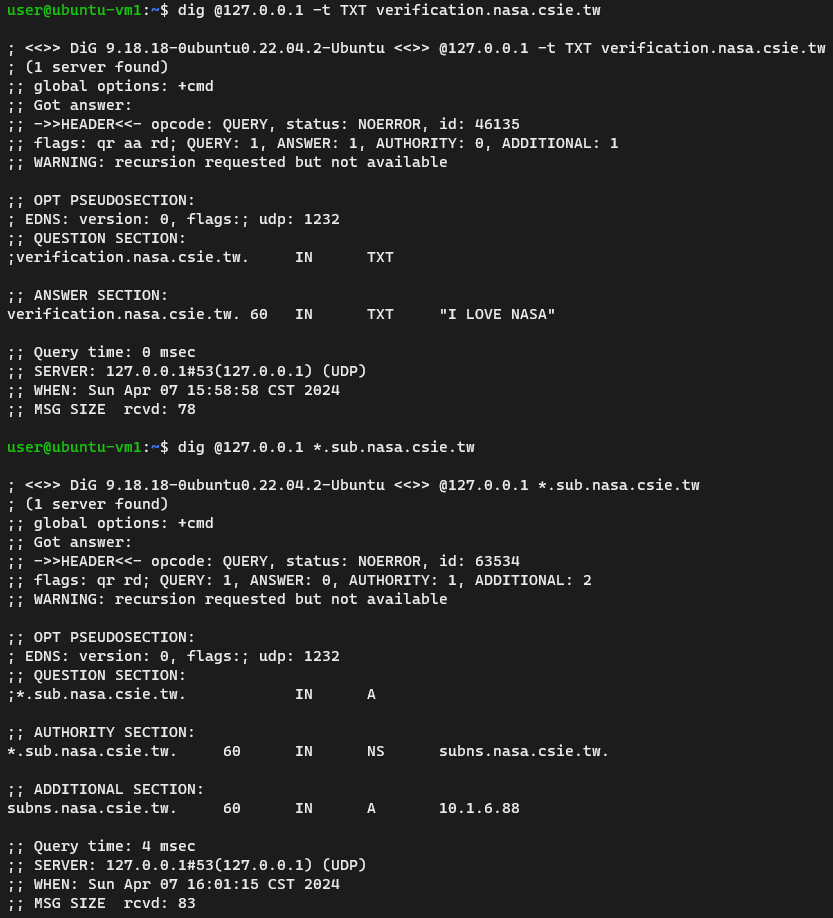
\includegraphics[width=0.93\textwidth]{4-3_dig.png}

    \textbf{References}
    \begin{itemize}
      \item \href{https://en.wikipedia.org/wiki/List_of_DNS_record_types}{List of DNS record types - Wikipedia}
      \item \href{https://www.cloudflare.com/learning/dns/dns-records/dns-ns-record/}{DNS NS record | Cloudflare}
    \end{itemize}
  \end{enumerate}
\end{document}
